%%% -*-LaTeX-*-

\chapter{NIC Aware Reconfiguration}
\label{chap:migration}
We have seen that the current generation of NICs are capable of transferring Gigabytes of 
data per second in latencies of the order of a few microseconds and we have reasons to believe 
that the next generation of networking hardware will have the ability to process 
hundreds of millions of messages per second at bandwidth of the order of tens of Gigabytes per 
second and sub microsecond latencies\cite{cx6}.
We saw from the previous chapters how the nuanced performance characteristics of 
a modern NIC will influence overall transmit performance and server resource utilisation 
for large data transfers such as responses to range scans. Yet another pressing 
concern for a modern In-memory database operating at scale is quick reconfiguration. 
Since DRAM is the most expensive resource in a modern cluster, efficient rebalancing 
involves fast reconfiguration that is frugal on resources and keeps the impact on their 
SLAs minimal. Informed with our lessons about the NIC, it is reasonable to assume that protocols for reconfiguration 
today can benefit from these optimisations and armed with the changes for proposed protocol, data migration might come 
closer to what the hardware is capable of doing today.

In this Chapter, we discuss the state of the art migration protocols and their 
performance, does an analysis of the existing migration protocol in RAMCloud, 
and armed with the lessons learned by profiling a modern NIC, we make concrete 
suggestions on how a new protocol might be well poised to take advantage of the 
new hardware.


\section{State of the art}
Fast reconfiguration of In-memory data is something that has been overlooked largerly
by the research community. There has been novel techniques for live migration of 
key value stores such as Albatross~\cite{albatross} which provides unavailability windows 
as short as 300ms, Zephyr~\cite{zephyr} which does on-demand pulls and asynchronous data 
pushes to minimize failed transactions and unavailability for migration while operating 
at transactional latencies of 50ms. Squall~\cite{squall} went further with fine grained 
partitioning with optimisations such as pre-fetching. Squall also offers minimal overhead 
to their transactional latencies which are of the order of tens of milliseconds and migrates 
data overall at the rate of around 5MB/s. While these efforts offer reconfiguration speeds 
better than other systems and minimal addition to their millisecond latencies, that is far 
from what a modern NIC is capable of delivering. From our benchmark, we knew that the NIC 
can deliver transmission throughputs of around 5GB/s while operating at microsecond latencies. 
There are important lessons to take from these recent research efforts on migration, but without 
devoting attention to the NIC and it's complex performance characteristics, today's cluster of
storage servers cannot offer migration performance order of magnitudes better than the state of the art.

\section{Migration in RAMCloud}
We saw from previous section what the latest reconfiguration protocols are capable of doing and how they can only 
offer 1000$\times$ less throughput than the latestoperating under millisecond latencies. There is a different class of systems~\cite{ramcloud,farm,rdmabillion,herd} that 
were developed recently which optimises for end-to-end latency and has the ability to perform millions of operations 
per second per server. RAMCloud~\cite{ramcloud} is a prime example of such a system which promises median read latencies 
of 5$\mu$s and responds to workloads upto a million operations per second. These characteristics result from the fact that 
these systems were designed from ground up keeping low latencies in mind and any significant disruption to their operating 
latencies might deem them less useful. RAMCloud has a migration protocol which offers around 100MB/s data transfer speeds albeit 
synchronous and unpipelined. While this is better by leaps and bounds than other systems, we believe that carefully leveraging the NIC, 
we can attain better throughput without compromising on latency.

\subsection{Current Protocol}
Figure ~\ref{fig:migration-current} shows the steps involved in the existing protocol. The key drawback to the current approach is that 
most of the steps involved are synchronous and blocking. The current protocol could make use of Zero Copy since migration usually involves 
large amount of data and sets of large data and the presence of \cpp{safeVersion}~\cite{ramcloudtx} makes Zero Copy an interesting proposition 
for migration in RAMCloud. While doing migrations, we found that the migration throughput that RAMCloud's existing protocol provides to 
be around 150MegaBytes per second (MB/s). While this is at least ten times better than the state of the art, there is definitely room for improvement in the protocol.
We profiled the time spent in migration doing each of the steps mentioned in Figure~\ref{fig:migration-current}.

\begin{figure}[t]
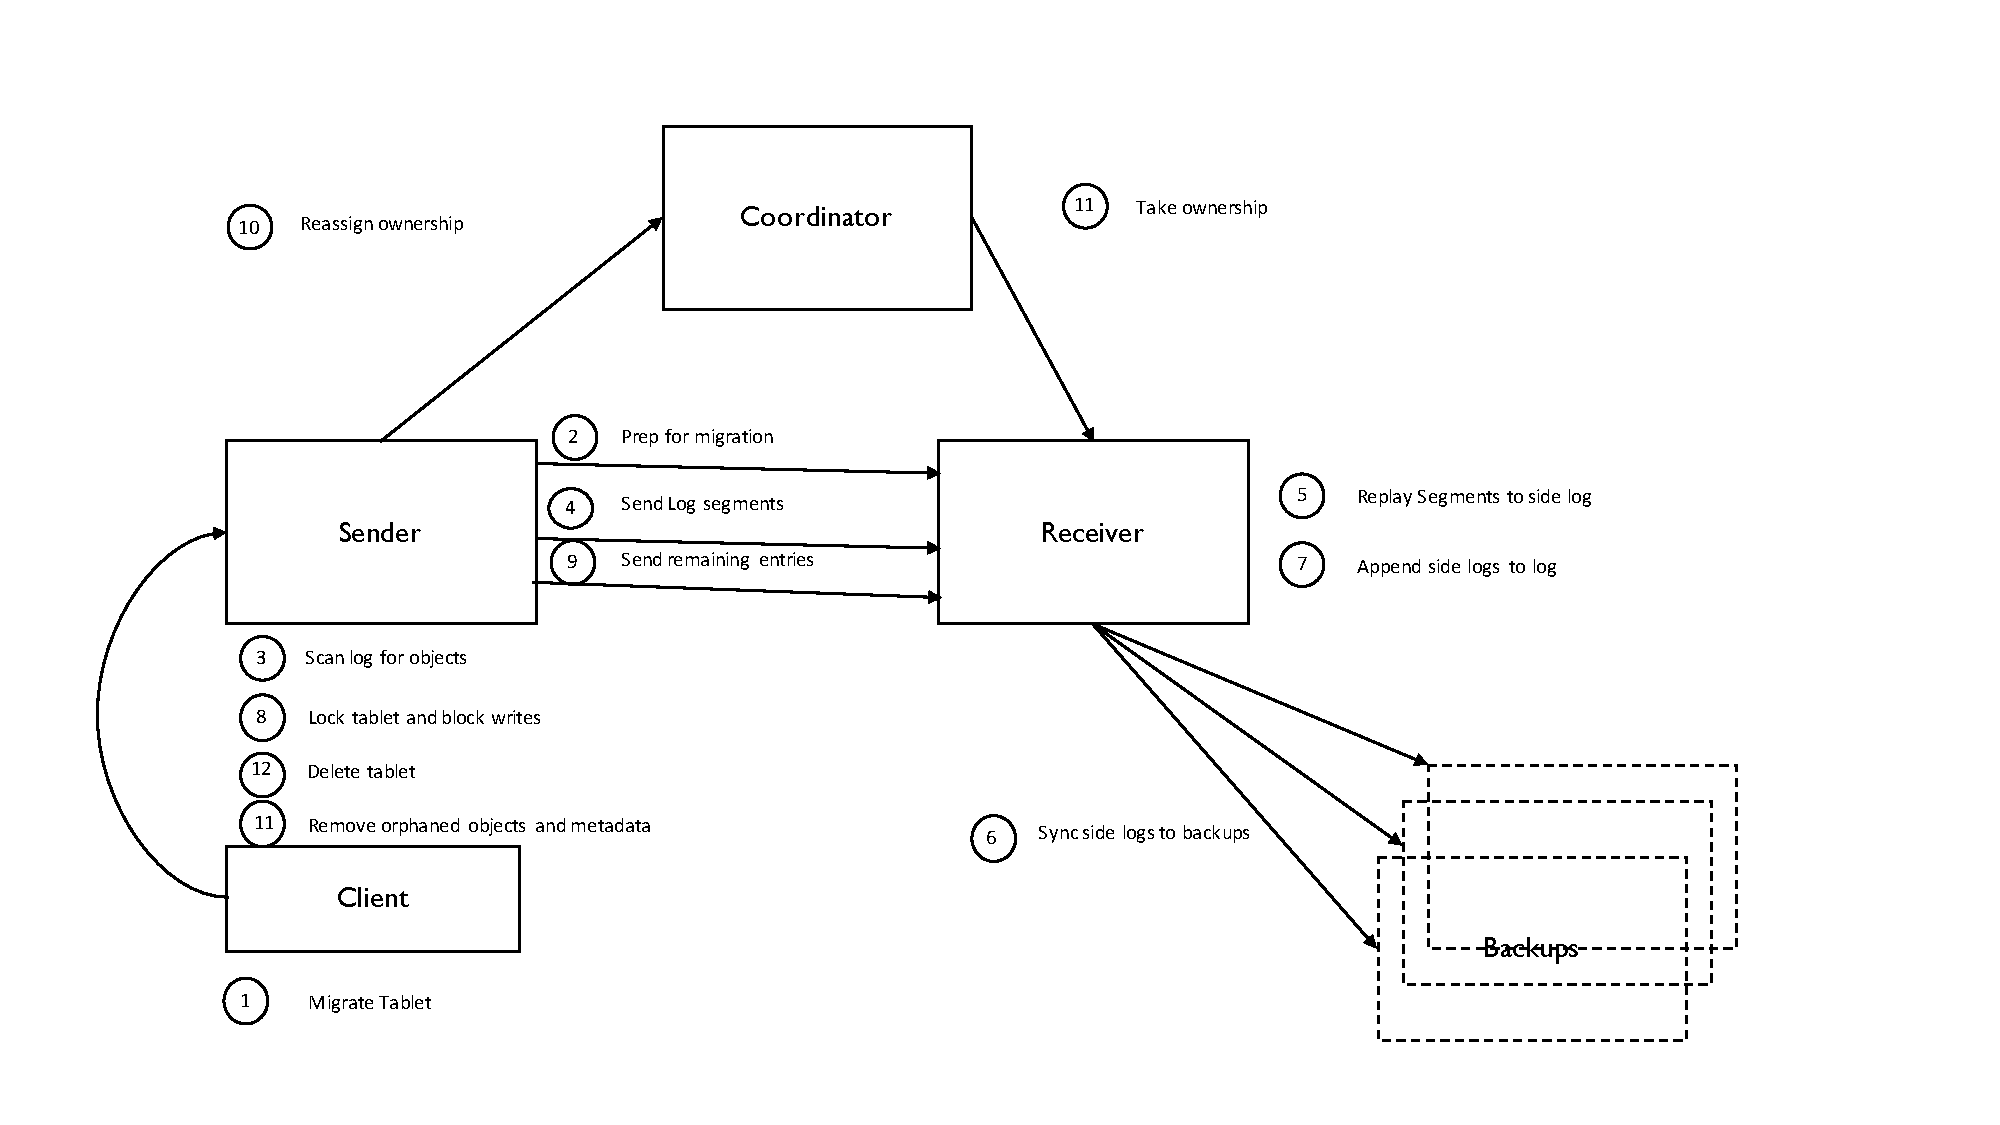
\includegraphics{fig-current-migration.pdf}
\caption{Diagram showing steps involved in the current migration protocol of RAMCloud}
\label{fig:migration-current}
\end{figure}


Figure~\ref{fig:bottlenecks} shows an analysis of how each of the bottlenecks affect RAMCloud's migration performance. We made versions of migration 
protocol bypassing each of the bottlenecks and measured RAMCloud's migration performance in each of those scenarios. We migrated a table of one million 
records with record sizes of 100~Bytes which comes close to ~150MB including the key and metadata.

The first bottleneck we bypassed was the re-replication of data to the backups. This is a configurable parameter and removing this we observed a speedup from around 150MB/s to around 
200MB/s. This explains that while disk bandwidth was indeed a bottleneck, avoiding it does not give significant performance boost while migrating a small data set.

The second bottleneck we tried to avoid was to skip replaying the migrated segments on the receiver. From here on, the safety of the protocol is heavily compromised even under 
 non failures. Since the point of the experiment was to show how much each step contributes to overall performance, we discard safety. Skipping replaying segments took us from 
 200MB/s to 600MB/s. 

Since we exhausted all steps involved in the receiver during migration, we skipped the actual transmission of data from source to destination and not surprisingly, the throughput 
only went up from 600MB/s to 700MB/s. 

The final step is the most interesting with respect to the lessons we have learned by analysing the NIC. Skipping the copying step before transmission took us from 700MB/s to 
1150MB/s. This underlines our earlier observation that any extra copy involved in a transmission is pure overhead and significantly affects performance. 

The analysis tells us that there is clearly room for improvement in migration performance in RAMCloud. While sequential replay of migrated segments of data seems to give the most benefits, 
it is safe to assume that use of Zero Copy while transmitting dat from source will definitely enhance network transmission throughput without hurting the available memory bandwidth.
\begin{figure}[t]
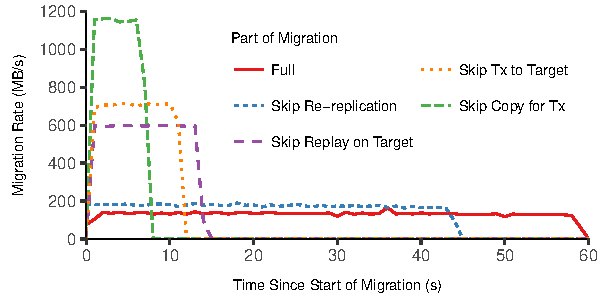
\includegraphics{fig-bottlenecks.pdf}
\caption{Bottleneck plot}
\label{fig:deltas}
\end{figure}


\subsection{Locality in RAMCloud}
RAMCloud's take on data locality is unique. RAMCloud promises uniform median latency of around 5$\mu$s~\cite{ramcloud}. RAMCloud doesn't have a strong notion of collocating data across servers. 
It is known that transactions~\cite{ramcloudtx} and secondary indices~\cite{SLIK} can benefit with collocation of data. RAMCloud data is hash partitioned and within a server, the in-memory log is organised 
in a temporal order. We might be tempted to think that storing data in contigous memory location in some order based on primary or secondary keys or even some other pre-determined order will give better NIC performance. 
The key obstruction to doing this is RAMCloud's log cleaning mechanism~\cite{ramcloudfast}. RAMCloud's design philosophy rightly highlights the importance of DRAM utilisation when all data is in memory. 
As a result, the log cleaner is designed in such a way that after cleaning, the log is reorganised so that records that are accessed in the same frequency are placed together, this makes sure that the records in the same 
segment gets garbage collected together freeing up more space than otherwise. To keep this property intact, we cannot force a deterministic order of data in RAMCloud and this might turn out to be a problem if 
we want to pre-aggregate data to get higher transmission throughput.

We set up an experiment to demonstrate the effect of collocating data in RAMCloud. RAMCloud's slated to provide a throughput of one million operations per second. We set up a cluster of 10 RAMCloud servers 
and had 10 client issue ``multiget'' requests to the servers which returns values for multiple keys in one operation. The operations were done on a table of 10 keys which were placed in various servers in different 
configuration. Figure~\ref{fig:colocation} shows the results from this experiment. When we had all 10 keys in one server, the whole cluster is expected to produce a throughput of 100 million objects read per second.
Owing to the overhead of multiget, we observe around 45 million combined operations on the server. The dotted line shows the throughput of the server if we were to use a regular ``get'' request to extract keys one by one.
We see a great benefit in the total throughput when all keys are collocated in a single server for all tables. The x-axis indicates the server spread. When we move along the x-axis, the second point indicates a configuration where for every table, 9 keys belong in one server and 
another belongs in a different server. The right most point is the configuration where each server hosts one key of all the 10 tables across the server. The bottom half explains what fraction of total CPU burned was spent 
doing useful work (worker) and what fraction went into handling the communication between servers(dispatch). We can cleary see that the amount of useful work done takes a great hit while the communication overhead dominates 
even if each server in the cluster had to do one cross-machine extraction of data. Adding this to the fact that if all the keys were evenly spread across the cluster, the ``multiget'' request does more harm than good and getting the 
keys one by one would've resulted in better aggregate throughput of the cluster, we can conclude that the effect of locality of data is paramount, and any movement of data to achieve better locality of data between servers will yield 
great performance later.

\begin{figure}[H]
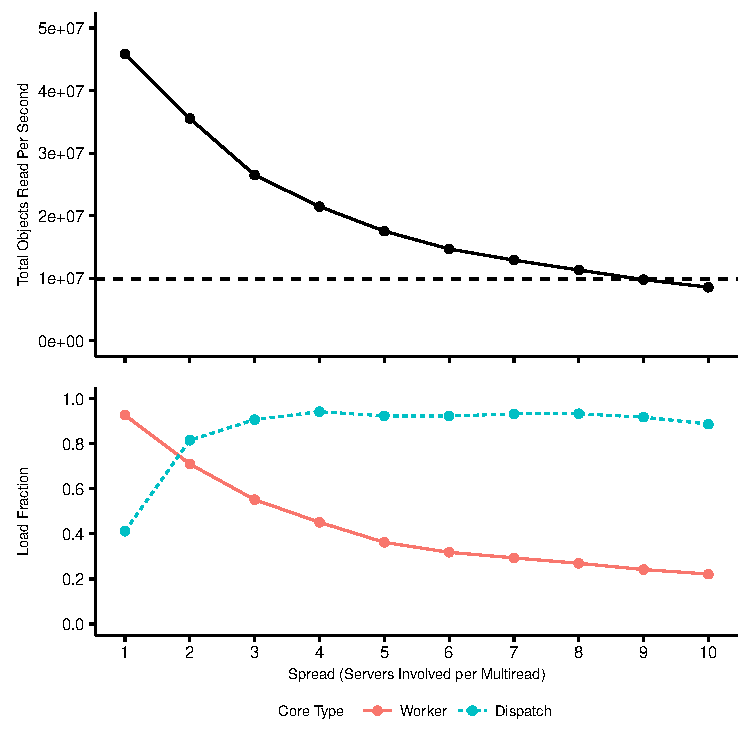
\includegraphics{fig-colocation.pdf}
\caption{Colocation plot}
\label{fig:colocation}
\end{figure}

\section{Design Guidelines for a new protocol}
Based on the analysis of the bottlenecks in the current protocol and the motivation that comes from having data localised to servers, some guidelines for developing a protocol for migration in RAMCloud
is given below which has ties to the lessons we learned from benchmarking a modern NIC.

\begin{itemize}
\item Make use of {\em Zero Copy}; RAMCloud supports a slew of network transport protocols including TCP and Infiniband. Since kernel by-pass is essential in the design philosophy which calls for minimal 
interrupts, more popular packet processing oriented transports like DPDK~\cite{dpdk} is also supported. No matter what protocol is used, We have seen from our previous chapters that 
using Zero Copy yields superior performance and efficient utilisation of resources. The new protocol should minimise the number of copies involved before transmission.

\item Layout your data such that there is {\em at least one large enough chunk} before transmission; Assuming we are doing a live migration while servicing data, it makes sense to reuse the principles of Bw-Trees here. Data 
could be pre-aggregated into a buffer and updates and some set of scattered records (limited by the network card) maybe transmitted giving near line rate throughput and minimal overhead to 
consumed memory bandwidth. Refer Section~\ref{sec:delta-tput-efficiency} for how a 16KB basepage can enhance transmission throughput by 1.6 times.

\item {\em Defer re-replication} to the end; Our analysis of experiments only showed minor increase of performance when we avoided re-replication. Larger migrations would need higher {\em disk I/O bandwidth} which gets bottlenecked at around 
300MB/s for regular spinning disks. It would be ideal to defer re-replication to the end provided there is some way to ensure safety of data in the face of failures during migration.

\item {\em Defer partitioning} decisions before migration; We mentioned that ordering data within a RAMCloud server is not feasible because of utilisation. Any new migration scheme should continue to adhere to the principle of assuming no locality 
of data within the server before migration unless significant changes are made to the log cleaning mechanism.

\item {\em Parallelise or pipeline} steps in migration; We saw from our analysis that the sequential nature of the migration is detrimental to it's performance. A new protocol should be 
able to parallelise the transfer of data as well as replaying at the receiver in order to attain maximum performance. 

\end{itemize}

